\begin{tikzpicture}[x=1bp,y=-1bp,line cap=round,line join=round]
\path[use as bounding box] (0,0) rectangle (770,270);
\begin{pgfinterruptboundingbox}
\draw[line width=2.5bp] (85,73) -- (727,73);
\draw[line width=2.5bp] (86,221) -- (184,221);
\draw[line width=2.5bp] (251,221) -- (728,221);
\draw[line width=2.5bp] (92,81) -- (91,213);
\draw[line width=2bp] (101,85) .. controls (112,109) and (115,129.0) .. (100,141.0);
\draw[line width=2bp] (100,151.0) .. controls (115,168.0) and (112,187) .. (101,208);
\node[inner sep=0pt,outer sep=0pt,rotate=0] at (72,52) {\scalebox{4}{\ensuremath{i}}};
\node[inner sep=0pt,outer sep=0pt,rotate=0] at (247,38) {\scalebox{4}{\ensuremath{1+i}}};
\node[inner sep=0pt,outer sep=0pt,rotate=0] at (62,140) {\scalebox{4}{\ensuremath{0}}};
\node[inner sep=0pt,outer sep=0pt,rotate=0] at (386,147) {\scalebox{3.65}{\textbf{Bereich für }$t$\textbf{ und }$\dfrac1t$}};
\end{pgfinterruptboundingbox}
\end{tikzpicture}
